\documentclass[]{article}
\usepackage{amsmath}
\usepackage{amsfonts}
\usepackage{amssymb}
\usepackage[retainorgcmds]{IEEEtrantools}
\usepackage{graphicx}
\usepackage{float}
%opening
\title{SVM and Email Classification}
\author{Samuel Schetterer}

\begin{document}

\maketitle
\clearpage

\section{Email Processing}
Email processing takes a few different steps:

\begin{itemize}
	\item Obtain a dataset of spam and not-spam emails to test the classifier against
	\item Clean undesireable content (actual emails, headers, etc) from the emails
	\item Tokenize and stem the emails
	\item Transform into some mathematical representation, here word vectors
\end{itemize}

\subsection{Dataset}

For 
These are easily available for download with little work.

The script I used for this can be found in the data/download\_email.sh folder

\subsection{Cleaning}
The emails are not immediately useful without some cleaning. They contain things like:


\begin{itemize}
	\item Email headers: "Received: from localhost (jalapeno [127.0.0.1])"
	\item Parsing the subject: "Subject: Lose weight now!"
	\item Urls: www.google.com
	\item Email addresses
	\item Punctuation
	\item Non-letter characters
	\item Stop words (and, the, ...)
\end{itemize}

We strip this content from the email. Urls are replaced with httpaddr, emails are replaced with emailaddr, and the rest is stripped.

The set of regexes and list of stop words used to clean the emails is in python/process\_email.py

\subsection{Tokenize}

We now tokenize and stem the emails. The stemming is nontrivial, since we want words like running and runs to map to the same stemmed word. For that, we use the porter-stemmer algorithm. There is an implementation provided with the Matlab source; however, since I don't have access to Matlab, I used the implementation from NLTK (https://github.com/nltk/nltk)

\subsection{Word Vectors}

To actually process the data, we need to turn it into a mathematical representation. This is done with the assistance of a vocabulary list provided with the project. For each stemmed word in the email, we see if there's a corresponding entry in the vocabularly list, and if so, add a vector with a 1 in the Nth dimension, where N is the number in the vocab list. This turns our problem into a mathematical problem with the dimension of our vocabulary list.

\subsection{Example stemming}

\textbf{We start with}

Hi,all:

Does anyone know how to list the biggest file in my
root directory?or the second biggest ..etc...

\textbf{Then after stripping it}

hiall anyone know list biggest file root directoryor second biggest etc

\textbf{And after stemming}

hiall anyon know list biggest file root directoryor second biggest etc

\noindent\rule[0.5ex]{\linewidth}{1pt}

Notably, this does not understand grammar and spelling mistakes in the emails - see directoryor for example.

\section{SVM mathematical model and examples}
The SVM is a mathematical model which tries to find an optimal separating plane between two datasets.

However, instead of worrying about the average distance, the SVM attempts only to reduce the distance between
the separating plane and the points closest to the plane - intuitively, this attempts to separate only based on the difficult to classify points instead of all of them.

This has a fortunate benefit of being easily expressible as a convex optimization problem:

We have some vector $\alpha$ and base point $\beta$ which describe our hyperplane, and some value $\omega$ which is the smallest distance froma point to the hyperplane. This is described by the minimization problem:

\subsection{Basic SVM}

\begin{equation}
\begin{split}
&\text{min: } -\omega
\\
&\text{s.t. } \alpha \cdot x_i - \beta <= \omega
\\
&\text{s.t. } \beta - \alpha \cdot y_i <= \omega
\\
&\text{s.t. } ||\alpha||_2 < K
\\
\end{split}
\end{equation}

Where $x$ is points in one class, $y$ is points in the other, and $K$ is an arbitrary positive constant, as is the choice of norm. This might generate a separating hyperplane like:

\begin{figure}[H]
	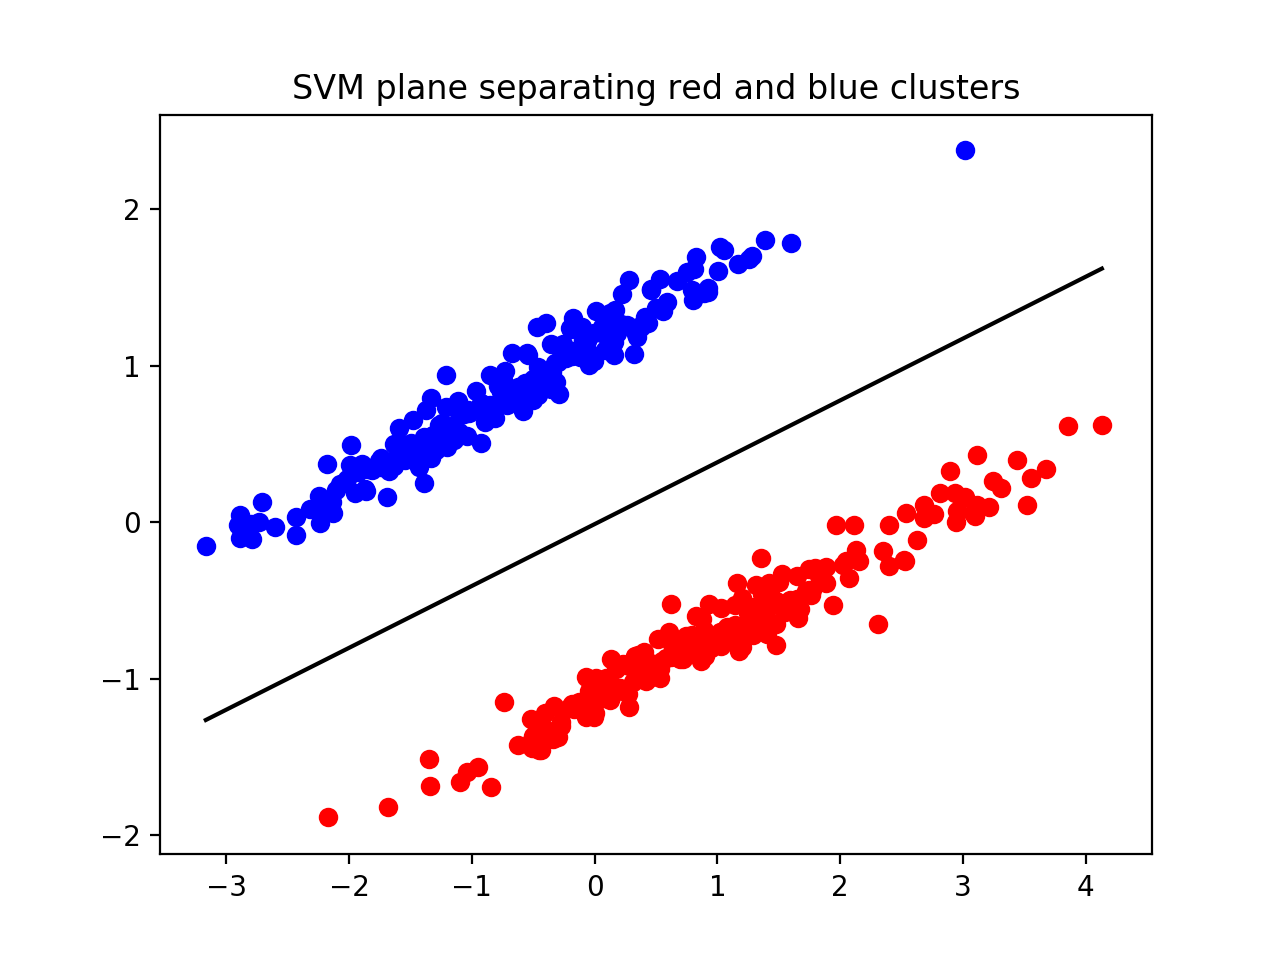
\includegraphics[width=\linewidth]{svm_low_var.png}
	\caption{Linearly separable datasets}
\end{figure}

\subsection{Nonseparable datasets}

While simple, this model has a massive downside - it can only work on linearly separable data. Otherwise, the constraints can't be satisfied. To get around this, we can introduce slack variables $\epsilon$ to  allow some give in the SVM. We also set the desired 'width' of the training set to 1, and allow the $\beta$ vector to vary for satisfying that constraint. This gives us:
	
	\begin{equation}
	\begin{split}
	&\text{min: } ||\epsilon_x||_1 + ||\epsilon_y||_1
	\\
	&\text{s.t. } \alpha \cdot x_i - \beta <= 1 - \epsilon_x
	\\
	&\text{s.t. } \beta - \alpha \cdot y_i  <= 1 - \epsilon_y
	\\
	&\text{s.t. } \epsilon_x > 0
	\\
	&\text{s.t. } \epsilon_y > 0
	\end{split}
	\end{equation}
	
With this model, we can fit non-separable data, like so (plotted with support planes for further analysis):

\begin{figure}[H]
	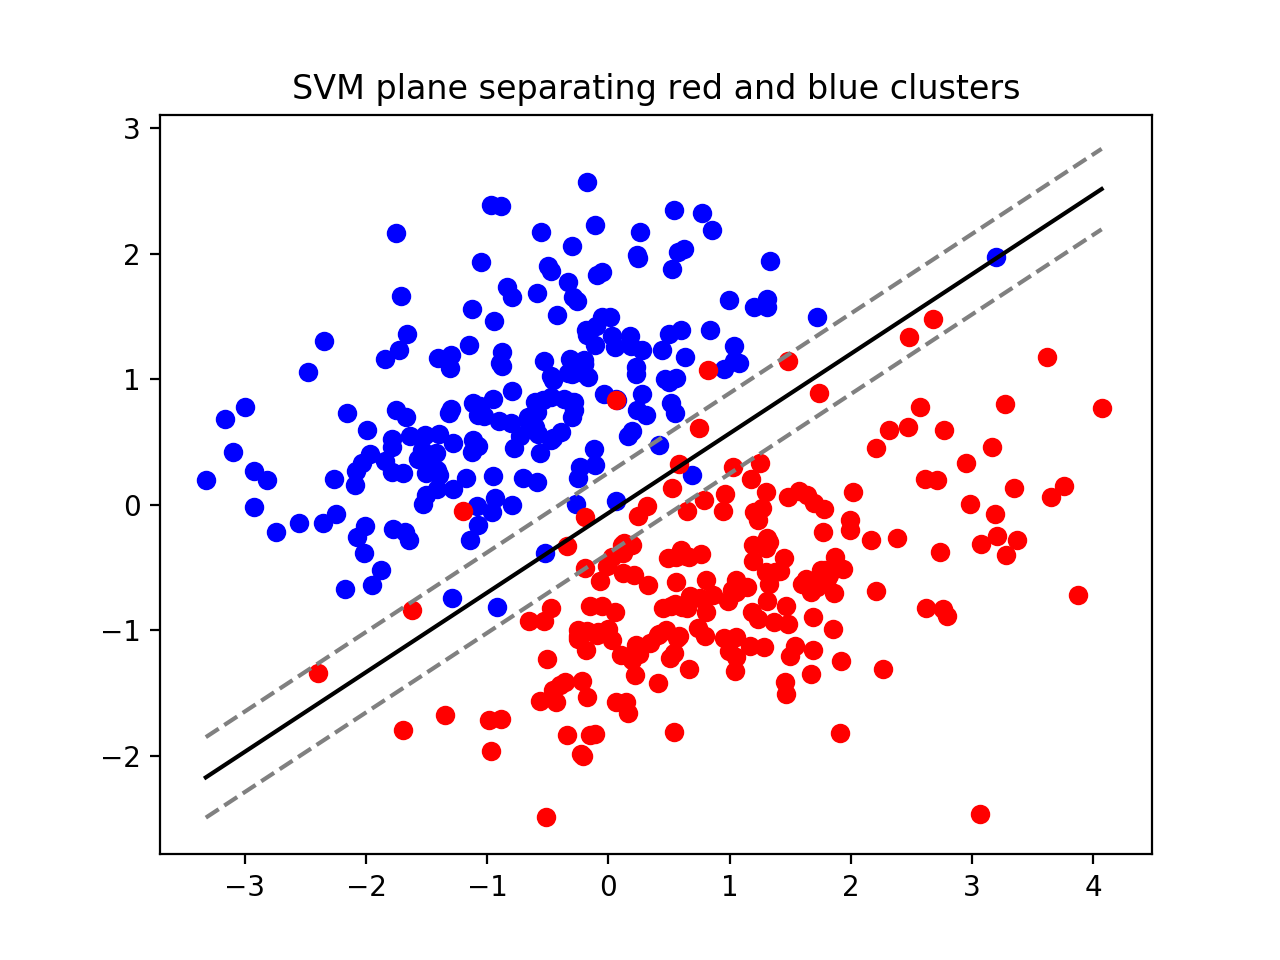
\includegraphics[width=\linewidth]{thin_lines.png}
	\caption{Non-separable datasets optimized for reduced slack}
\end{figure}

We can see that the model fits, and with the plotted support planes, that this optimizes to shrink the required slack variable.


\subsection{Beta regularization}

This model has one last problem - it aggressively optimizes to fit a perfect line, and will create arbitrarily large $\beta$ vectors to
reduce the slack needed. To solve that, we add a term in the objective which punishes a large $\beta$:

\begin{equation}
\begin{split}
&\text{min: } ||\epsilon_x||_1 + ||\epsilon_y||_1 + ||\beta||_2
\\
&\text{s.t. } \alpha \cdot x_i - \beta <= 1 - \epsilon_x
\\
&\text{s.t. } \beta - \alpha \cdot y_i  <= 1 - \epsilon_y
\\
&\text{s.t. } \epsilon_x > 0
\\
&\text{s.t. } \epsilon_y > 0
\end{split}
\end{equation}

This provides a tunable balance between fitting the outliers well (low slack variable) and reducing the variance(smaller $\beta$).

Looking at the svm, we can see that with a beta regularization term, the supporting vectors are less accurate, although the model will have less variance with the training data.

\begin{figure}[H]
	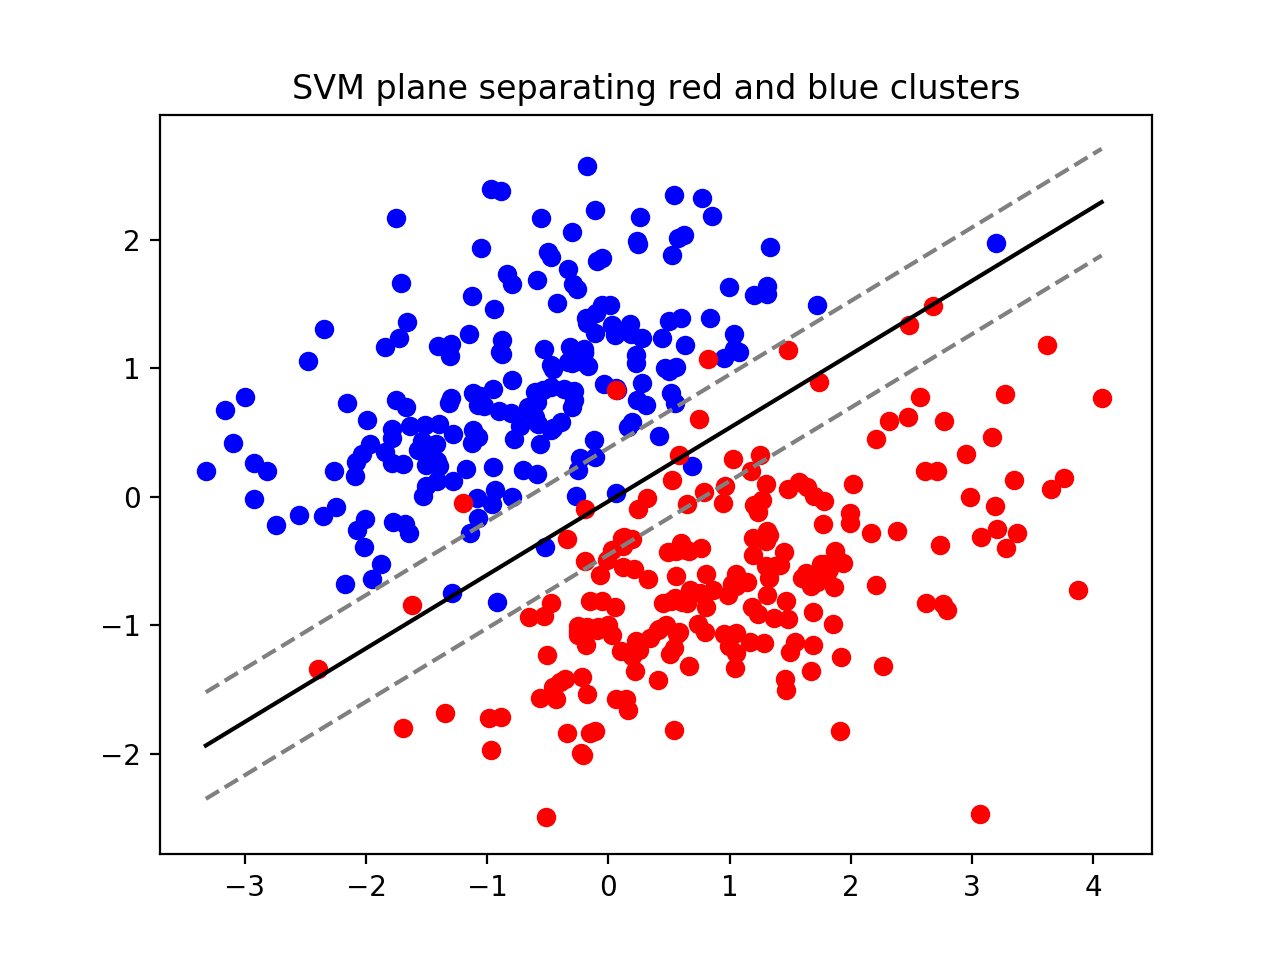
\includegraphics[width=\linewidth]{thick_lines.png}
	\caption{Non-separable datasets with $\beta$ regularization}
\end{figure}

\section{Results on email spam}
When training the email on the downloaded datasets, I randomly select 1/5 of the data to use for training and use the rest as a test dataset. The random seed is passed to the report as a parameter to ensure reproducibility.

I also test on the downloaded dataset without the hard non-spam emails, to see if those affect spam accuracy, considering the full downloaded dataset (Hard), and the downloaded set with only easy emails (Easy)

The results are as follows for training and test data:

\begin{table}[H]
	\begin{center}
		\caption{SVM accuracy (\% correct) on downloaded and provided email datasets for training data}
		\label{tab:table1}
		\begin{tabular}{|lr|r|r} % <-- Alignments: 1st column left, 2nd middle and 3rd right, with vertical lines in between
			\textbf{Group} & \textbf{Ham} & \textbf{Spam} & \textbf{Total}\\
			\hline
			Hard & 100 & 100 & 100 \\
			Easy & 99.7 & 100 & 99.8 \\
			Provided & 100 & 100 & 100 \\
		\end{tabular}
	\end{center}
\end{table}

\begin{table}[H]
\begin{center}
	\caption{SVM accuracy (\% correct) on downloaded and provided email datasets for test data}
	\label{tab:table1}
	\begin{tabular}{|lr|r|r} % <-- Alignments: 1st column left, 2nd middle and 3rd right, with vertical lines in between
		\textbf{Group} & \textbf{Ham} & \textbf{Spam} & \textbf{Total}\\
		\hline
		Hard & 97.4 & 93.0 & 96.0 \\
		Easy & 97.0 & 94.5 & 96.0 \\
		Provided & 96.4 & 97.8 & 97.4 \\
	\end{tabular}
\end{center}
\end{table}

The linear SVM model does extremely well here on the test datasets, all with overall accuracy above 95\%. It's safe to conclude that the datasets are almost linearly seperable, and that a linear SVM model is capable of effectively classifing spam vs not-spam emails, at least those which resemble the passed dataset.

\section{Future work}
There are a a few interesting directions to take this classifier that I didn't have time to complete or didn't have luck with.

\subsection{Biased SVM}

One considers the problem "How can I make the decision boundary favor one class over another, at the potential cost of accuracy"?

I investigated modifying the objective as such, with $0 < \theta < 1$

\begin{equation}
\begin{split}
&\text{min: } \theta||\epsilon_x||_1 + (1 - \theta)||\epsilon_y||_1 + ||\beta||_2
\\
&\text{s.t. } \alpha \cdot x_i - \beta <= 1 - \epsilon_x
\\
&\text{s.t. } \beta - \alpha \cdot y_i  <= 1 - \epsilon_y
\\
&\text{s.t. } \epsilon_x > 0
\\
&\text{s.t. } \epsilon_y > 0
\end{split}
\end{equation}

The goal was to punish slack variables relative to the 'innaccurate class', as to encourage missclassifying one class in favor of the other. This might be desireable in something like spam classification, where one cares much more about letting real emails through  as opposed to catching all of the spam.

However, when training with this model, I got the extremely unintuitive result where punishing the slack variables for a class moved the support boundary towards that class, instead of away from it as expected. I ran out of time investigating this issue unfortunately, but suspect it would have many uses in real life.

\subsection{Dimensionality reduction}

Currently, the size of our dataset is rather small compared to the number of dimension, each a similar order of magnitude. It's very likely that this dataset is extremely sparse, and most emails could be well represented in a lower dimensional dataset.

If this were the case, one would be in a better position to examine more sophisticated SVM algorithms operating on this low dimensional representation.

\subsection{Partial email examination}

II suspect it's likely that the spam-ness of an email can be determined from only the first few words (I certainly can do it well on my own emails). Training an accurate SVM on just the first few words could be useful in a performance sensitive environment, so one can ignore most of the email and save resources.

For spam classification, there could be a pre-classifier which identifies possible spam emails to analyze more closely, while skipping most of the analysis on most emails.

I didn't carry this out in the project because of some problems I had with my email processing implementation, which led to me using the provided training matrices for most of the project.

\section{External code}

NLTK: https://github.com/nltk/nltk, used for stop word list and porter-stemmer
CVXPY: https://www.cvxpy.org/, used as optimization interface
StackOverflow: https://stackoverflow.com/, used for many minor coding questions

\section{Citations}

C.J. van Rijsbergen, S.E. Robertson and M.F. Porter, 1980. New models in probabilistic information retrieval. London: British Library. (British Library Research and Development Report, no. 5587).

\end{document}